\section{Survival analysis}

\subsection{Time and censoring}

For an anchor \(i\) whose successor \(\hat{j}_i\) is accepted:
\[\tau_i = v_{\hat{j}_i} - u_i, \qquad Y_i = 1.\]
If no successor is accepted before 31 December 2025:
\[\tau_i = \text{2025-12-31} - u_i, \qquad Y_i = 0,\]
and the row is \textbf{administratively right-censored}. Time zero is the award date.

The cohort therefore holds \textbf{3,800 awarded procurement episodes, 544 events and 3,256 censored observations} (85.7 \%). That high censoring rate is precisely why survival analysis is used rather than a regression on linked episodes alone: ignoring censoring would restrict the analysis to episodes whose successor has been seen, that is, condition the analysis on the outcome.

\subsection{Non-parametric estimation}

The Kaplan--Meier estimator \citep{kaplan1958},
\[\hat S(t) = \prod_{t_k \le t}\left(1 - \frac{d_k}{n_k}\right),\]
with \(d_k\) events at \(t_k\) and \(n_k\) at risk, assumes no distributional form and handles administrative censoring without bias as long as censoring is independent of the hazard.

\begingroup\footnotesize
\begin{longtable}[]{@{}lrr@{}}
\toprule\noalign{}
Horizon & P(observable successor) & Survival \\
\midrule\noalign{}
\endhead
\bottomrule\noalign{}
\endlastfoot
12 months & \textbf{4.62 \%} & 0.9538 \\
24 months & \textbf{6.73 \%} & 0.9327 \\
36 months & 8.68 \% & 0.9132 \\
48 months & 15.50 \% & 0.8450 \\
60 months & 17.54 \% & 0.8246 \\
\end{longtable}
\endgroup

\textbf{The Kaplan-Meier median is not reached}: the curve never falls below 0.5 within the observation window. The 31.8 months quoted elsewhere is the median \emph{among linked events only}; the two quantities share a word and measure different things, the second being conditional on the event having occurred.

The jump between 36 and 48 months --- 8.7 \% to 15.5 \% --- is the \textbf{re-procurement shoulder}. Its timing is compatible with multi-year purchasing cycles, but the event is an observable successor and does not establish a legal renewal.

\begin{figure}[htbp]
\centering
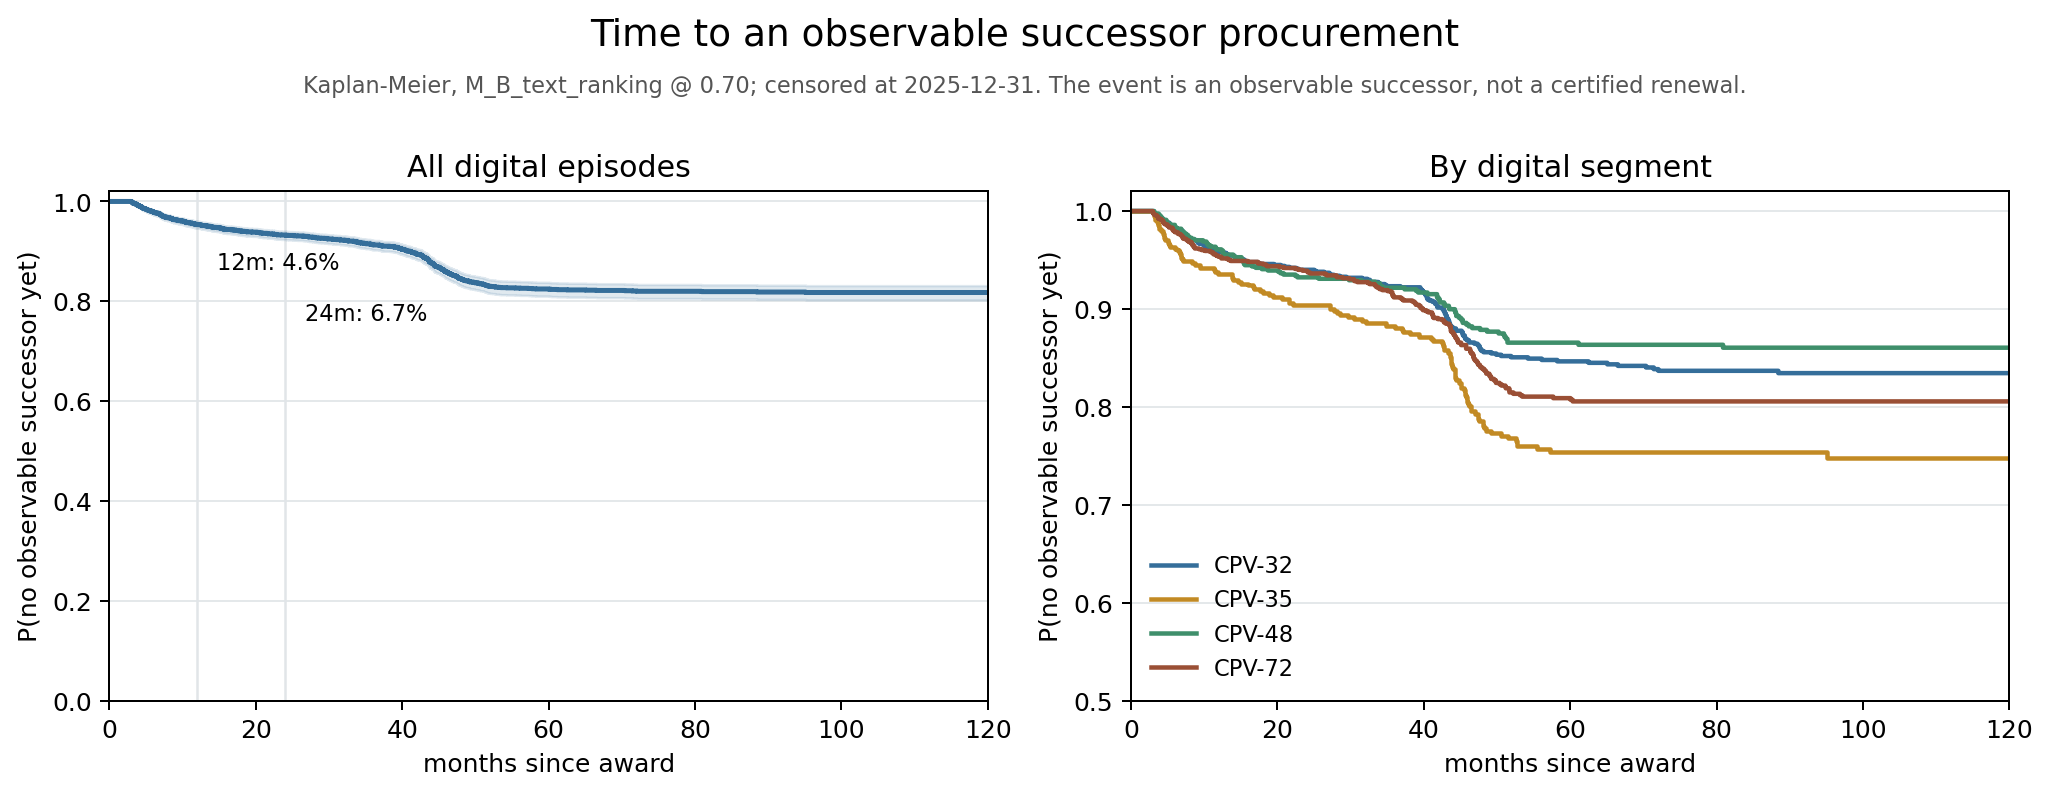
\includegraphics[width=1.0\linewidth]{figures/fig02_km_overall_and_segment.png}
\caption{Time to an observable successor procurement under the frozen \texttt{M\_B @ 0.70} rule, censored at 2025-12-31. Left: the whole cohort; the curve never falls below 0.5, so the Kaplan--Meier median is not reached, and the drop sits between 40 and 48 months. Right: by CPV division; CPV-35 separates from the other three. \textbf{The right-hand axis starts at 0.5, not 0}, so the separation appears larger than on the full scale. At-risk counts are in Annex D.}
\label{fig:km}
\end{figure}
 It is the most interesting part of the curve for Gigalis and also the most fragile: at 48 months the risk set contains only pre-2022 awards, so cohort composition changes along the curve. It should not be quoted without the at-risk counts (Annex D).

\textbf{Between-segment comparison.} The multivariate log-rank test across the four CPV segments gives a statistic of \textbf{23.45} for \(p = 3.3\times 10^{-5}\): the segments do not behave alike. Raw event rates run from 11.6 \% (CPV-48) to 20.4 \% (CPV-35).

\subsection{Conditional probabilities: the operational output}

For a procurement episode that has reached age \(a\) with no observed successor, the probability that one appears within the next \(h\) months is
\[P(T \le a+h \mid T > a) = 1 - \frac{S(a+h)}{S(a)},\]
read off the Kaplan-Meier estimator. Both 500-draw episode-bootstrap and buyer-cluster-bootstrap intervals are reported; the latter resamples buyers and preserves the dependence among their episodes.

\begingroup\footnotesize
\begin{longtable}[]{@{}
  >{\raggedleft\arraybackslash}p{(\columnwidth - 8\tabcolsep) * \real{0.2222}}
  >{\raggedleft\arraybackslash}p{(\columnwidth - 8\tabcolsep) * \real{0.2222}}
  >{\raggedright\arraybackslash}p{(\columnwidth - 8\tabcolsep) * \real{0.1667}}
  >{\raggedleft\arraybackslash}p{(\columnwidth - 8\tabcolsep) * \real{0.2222}}
  >{\raggedright\arraybackslash}p{(\columnwidth - 8\tabcolsep) * \real{0.1667}}@{}}
\toprule\noalign{}
\begin{minipage}[b]{\linewidth}\raggedleft
Episode age
\end{minipage} & \begin{minipage}[b]{\linewidth}\raggedleft
P(successor $\le$ 12 m)
\end{minipage} & \begin{minipage}[b]{\linewidth}\raggedright
95 \% CI (episode; buyer)
\end{minipage} & \begin{minipage}[b]{\linewidth}\raggedleft
P($\le$ 24 m)
\end{minipage} & \begin{minipage}[b]{\linewidth}\raggedright
95 \% CI (episode; buyer)
\end{minipage} \\
\midrule\noalign{}
\endhead
\bottomrule\noalign{}
\endlastfoot
0 months & 4.62 \% & {[}3.91; 5.24{]}; {[}3.63; 5.68{]} & 6.73 \% & {[}5.91; 7.58{]}; {[}5.25; 8.59{]} \\
12 months & 2.22 \% & {[}1.70; 2.73{]}; {[}1.38; 3.23{]} & 4.26 \% & {[}3.55; 4.98{]}; {[}3.25; 5.36{]} \\
24 months & 2.09 \% & {[}1.58; 2.60{]}; {[}1.54; 2.63{]} & 9.40 \% & {[}8.33; 10.68{]}; {[}7.69; 11.20{]} \\
\textbf{36 months} & \textbf{7.46 \%} & {[}6.52; 8.59{]}; {[}5.88; 9.06{]} & \textbf{9.69 \%} & {[}8.58; 11.12{]}; {[}7.88; 11.71{]} \\
48 months & 2.41 \% & {[}1.77; 3.07{]}; {[}1.66; 3.32{]} & 2.89 \% & {[}2.15; 3.72{]}; {[}2.08; 3.91{]} \\
\end{longtable}
\endgroup

The profile is not monotone in age: it rises into the 36-48 month shoulder and falls away after it. Buyer clustering widens several intervals but does not materially change this operational pattern. The table is therefore used as a \textbf{cohort-level watch logic}: it ranks ages and segments, it does not predict an individual episode.

\begin{figure}[htbp]
\centering
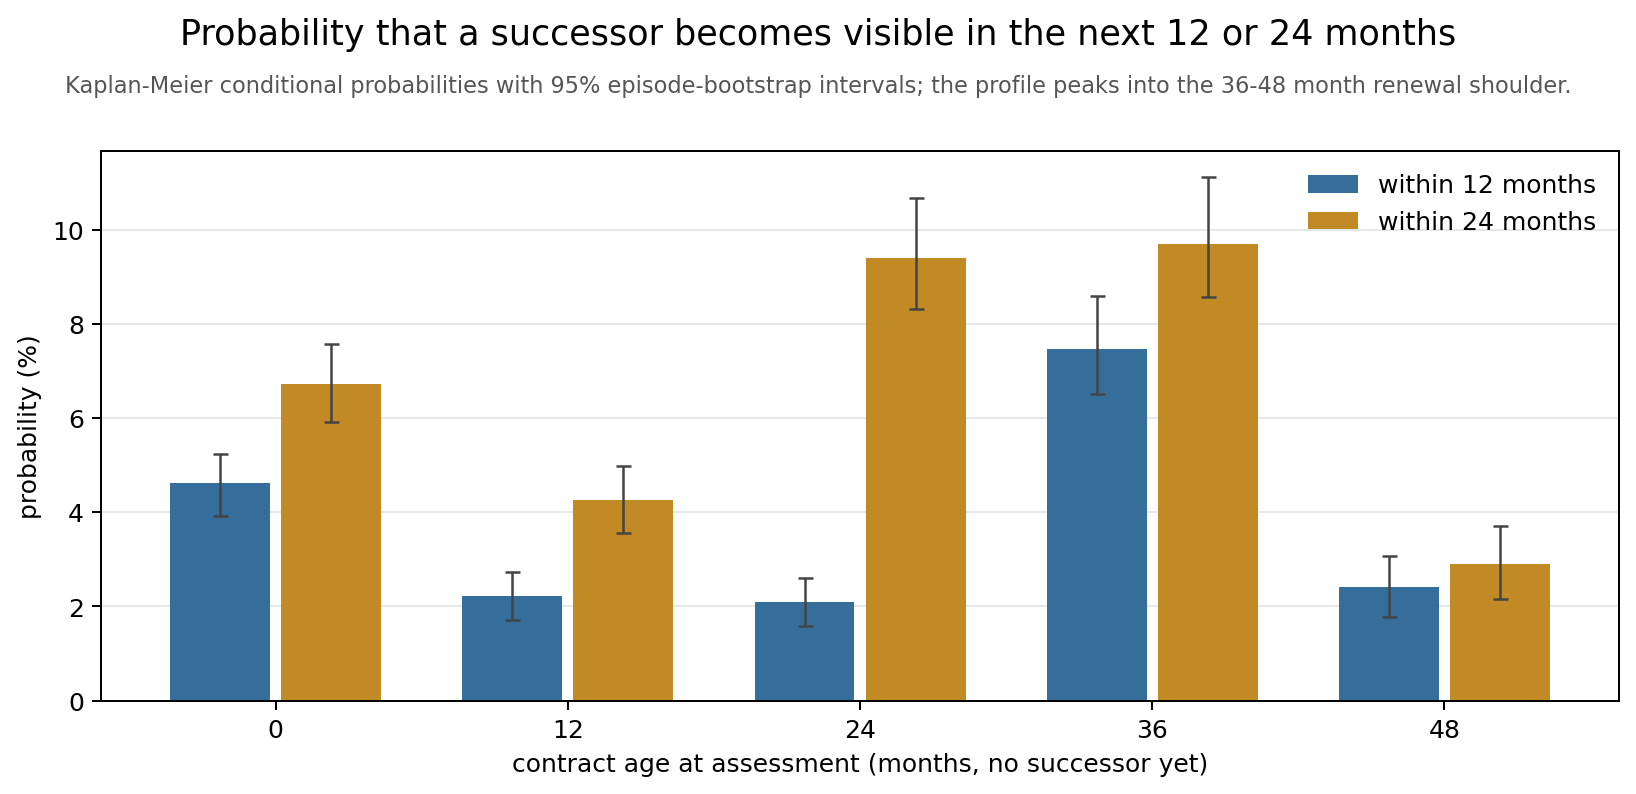
\includegraphics[width=0.85\linewidth]{figures/fig03_conditional_probabilities.png}
\caption{Probability that an observable successor appears within the next 12 or 24 months, by episode age, with 500-draw episode-bootstrap intervals. Buyer-cluster intervals are reported in the table and are somewhat wider without changing the pattern. The profile peaks around 36 months and falls away afterwards; it supports cohort-level monitoring, not individual prediction.}
\label{fig:condprob}
\end{figure}


\subsection{Cox model: comparative associations}

The proportional-hazards model \citep{cox1972},
\[h(t \mid X) = h_0(t)\exp(\beta_1X_1 + \cdots + \beta_pX_p),\]
estimates covariate effects without specifying the baseline hazard. Five covariates are retained, consistent with the one-parameter-per-ten-events rule: CPV segment, region, framework status, validated-SIREN availability, and centred award year --- eight parameters for 544 events.

\begingroup\small
\begin{longtable}[]{@{}
  >{\raggedright\arraybackslash}p{(\columnwidth - 6\tabcolsep) * \real{0.2143}}
  >{\raggedleft\arraybackslash}p{(\columnwidth - 6\tabcolsep) * \real{0.2857}}
  >{\raggedright\arraybackslash}p{(\columnwidth - 6\tabcolsep) * \real{0.2143}}
  >{\raggedleft\arraybackslash}p{(\columnwidth - 6\tabcolsep) * \real{0.2857}}@{}}
\toprule\noalign{}
\begin{minipage}[b]{\linewidth}\raggedright
Covariate
\end{minipage} & \begin{minipage}[b]{\linewidth}\raggedleft
HR
\end{minipage} & \begin{minipage}[b]{\linewidth}\raggedright
95 \% CI
\end{minipage} & \begin{minipage}[b]{\linewidth}\raggedleft
p
\end{minipage} \\
\midrule\noalign{}
\endhead
\bottomrule\noalign{}
\endlastfoot
Framework agreement & 1.751 & {[}1.435; 2.136{]} & $3.4\times 10^{-8}$ \\
\textbf{CPV-35} (ref. CPV-32) & \textbf{1.553} & {[}1.218; 1.981{]} & \textbf{$3.8\times 10^{-4}$} \\
CPV-48 & 0.828 & {[}0.638; 1.073{]} & 0.153 \\
CPV-72 & 1.056 & {[}0.850; 1.310{]} & 0.624 \\
Normandie (ref. Bretagne) & 0.800 & {[}0.640; 1.000{]} & 0.050 \\
Pays de la Loire & 1.003 & {[}0.815; 1.234{]} & 0.979 \\
Validated SIREN & 1.082 & {[}0.885; 1.323{]} & 0.443 \\
Award year (centred) & 1.107 & {[}1.066; 1.149{]} & $1.2\times 10^{-7}$ \\
\end{longtable}
\endgroup

In-sample concordance: 0.626.

This population model answers how episodes compare across the Grand Ouest cohort. In that estimand, CPV-35 episodes show earlier observable successors (HR 1.553). It is a descriptive population contrast, not an intrinsic or causal segment effect; the within-buyer sensitivity below answers a different question and attenuates this estimate.

The assumption is tested on weighted Schoenfeld residuals \citep{grambsch1994}. \textbf{The diagnostic rejects constant effects for three covariates}: award year (statistic 70.7, \(p = 4\times 10^{-17}\)), framework status (7.04, \(p = 0.008\)) and validated SIREN (6.76, \(p = 0.009\)). The award-year violation is severe and expected: award year is structurally confounded with follow-up length. These coefficients are therefore \textbf{time-averaged descriptive associations, not effects}. Stratifying on award-year bands would be cleaner; it was judged optional because the coefficients of interest barely move and nothing operational rests on this model.

\subsection{Temporal validation: a negative result}

The model is fitted once on 2015-2021 awards and scored out of time, with no refitting and no retuning.

\begingroup\footnotesize
\begin{longtable}[]{@{}
  >{\raggedright\arraybackslash}p{(\columnwidth - 12\tabcolsep) * \real{0.1111}}
  >{\raggedleft\arraybackslash}p{(\columnwidth - 12\tabcolsep) * \real{0.1481}}
  >{\raggedleft\arraybackslash}p{(\columnwidth - 12\tabcolsep) * \real{0.1481}}
  >{\raggedleft\arraybackslash}p{(\columnwidth - 12\tabcolsep) * \real{0.1481}}
  >{\raggedleft\arraybackslash}p{(\columnwidth - 12\tabcolsep) * \real{0.1481}}
  >{\raggedleft\arraybackslash}p{(\columnwidth - 12\tabcolsep) * \real{0.1481}}
  >{\raggedleft\arraybackslash}p{(\columnwidth - 12\tabcolsep) * \real{0.1481}}@{}}
\toprule\noalign{}
\begin{minipage}[b]{\linewidth}\raggedright
Window
\end{minipage} & \begin{minipage}[b]{\linewidth}\raggedleft
Train N
\end{minipage} & \begin{minipage}[b]{\linewidth}\raggedleft
Train events
\end{minipage} & \begin{minipage}[b]{\linewidth}\raggedleft
Test N
\end{minipage} & \begin{minipage}[b]{\linewidth}\raggedleft
Test events
\end{minipage} & \begin{minipage}[b]{\linewidth}\raggedleft
Train C
\end{minipage} & \begin{minipage}[b]{\linewidth}\raggedleft
\textbf{Test C}
\end{minipage} \\
\midrule\noalign{}
\endhead
\bottomrule\noalign{}
\endlastfoot
Primary, 2022-2024 & 2,470 & 392 & 1,004 & 107 & 0.606 & \textbf{0.479} \\
Sensitivity, 2022-2025 & 2,470 & 392 & 1,330 & 152 & 0.606 & \textbf{0.518} \\
\end{longtable}
\endgroup

A concordance point estimate of 0.479 is close to chance. A fixed-prediction bootstrap gives an episode-level 95\,\% interval of {[}0.415; 0.542{]} and a wider buyer-cluster interval of {[}0.360; 0.634{]}, reflecting dependence among episodes from the same buyer. The available temporal validation therefore \textbf{does not establish useful individual discrimination}; it does not mathematically rule out every moderately discriminative population value. Part of the difficulty is structural --- episodes awarded from 2022 can only contribute short gaps, and Harrell's C \citep{harrell1982} depends on the censoring distribution \citep{uno2011}, so two windows with unequal follow-up are not strictly comparable.

The result is published as it stands, and it drives a decision: \textbf{the Cox model is not used as an individual ranking engine}. The brief expected a table of the twenty contracts most likely to be renewed; producing it would convey a precision the validation does not support. The operational deliverable is therefore the conditional table of \S~5.3 and, in the annex, a \textbf{segment-stratified watch list} --- five episodes per CPV segment among those awarded since 2021 --- read off the segment-stratified Kaplan-Meier curves rather than the Cox model. The stratification is deliberate: since the conditional probability is a function of segment and age alone, a global ranking would mechanically return the highest-hazard segment at the age closest to the shoulder, implying an individual-level granularity that does not exist.

\subsection{Parametric models}

Five accelerated-failure-time families \citep{kalbfleisch2002} were fitted and compared on AIC and BIC:

\begingroup\footnotesize
\begin{longtable}[]{@{}lrrrr@{}}
\toprule\noalign{}
Model & Parameters & Log-likelihood & AIC & BIC \\
\midrule\noalign{}
\endhead
\bottomrule\noalign{}
\endlastfoot
\textbf{Generalised gamma} & 3 & $-$3,757.5 & \textbf{7,521.0} & \textbf{7,539.7} \\
Log-normal & 2 & $-$3,784.6 & 7,573.2 & 7,585.7 \\
Log-logistic & 2 & $-$3,807.3 & 7,618.6 & 7,631.1 \\
Weibull & 2 & $-$3,814.7 & 7,633.4 & 7,645.8 \\
Exponential & 1 & $-$3,829.7 & 7,661.3 & 7,667.6 \\
\end{longtable}
\endgroup

The generalised gamma wins on both criteria. It is \textbf{not} the source of the operational figures, and that choice deserves defending: every one of these families is smooth and flattens the empirical 36-48 month shoulder, which is precisely the business object; and every published horizon (12, 24 months) lies inside the observed window, where the empirical estimator needs no shape assumption. The parametric model is therefore kept as the best-fitting family and as the instrument any extrapolation beyond 31 December 2025 would use. Mechanically taking the lowest AIC to produce operational numbers would have traded a slightly better global fit for a worse rendering of the only region the user cares about.

\subsection{Robustness and sensitivity checks}

This is the most important section of the report for interpretation, because it separates what moves from what holds.

\textbf{(a) Four event definitions.}

\begingroup\footnotesize
\begin{longtable}[]{@{}
  >{\raggedright\arraybackslash}p{(\columnwidth - 10\tabcolsep) * \real{0.1304}}
  >{\raggedleft\arraybackslash}p{(\columnwidth - 10\tabcolsep) * \real{0.1739}}
  >{\raggedleft\arraybackslash}p{(\columnwidth - 10\tabcolsep) * \real{0.1739}}
  >{\raggedleft\arraybackslash}p{(\columnwidth - 10\tabcolsep) * \real{0.1739}}
  >{\raggedleft\arraybackslash}p{(\columnwidth - 10\tabcolsep) * \real{0.1739}}
  >{\raggedleft\arraybackslash}p{(\columnwidth - 10\tabcolsep) * \real{0.1739}}@{}}
\toprule\noalign{}
\begin{minipage}[b]{\linewidth}\raggedright
Arm
\end{minipage} & \begin{minipage}[b]{\linewidth}\raggedleft
Events
\end{minipage} & \begin{minipage}[b]{\linewidth}\raggedleft
Rate
\end{minipage} & \begin{minipage}[b]{\linewidth}\raggedleft
P($\le$ 12 m)
\end{minipage} & \begin{minipage}[b]{\linewidth}\raggedleft
P($\le$ 24 m)
\end{minipage} & \begin{minipage}[b]{\linewidth}\raggedleft
Median observed gap
\end{minipage} \\
\midrule\noalign{}
\endhead
\bottomrule\noalign{}
\endlastfoot
\texttt{M\_B\ @\ 0.80} strict & 296 & 7.8 \% & 2.37 \% & 3.23 \% & 35.7 months \\
\textbf{\texttt{M\_B\ @\ 0.70} primary} & \textbf{544} & \textbf{14.3 \%} & \textbf{4.62 \%} & \textbf{6.73 \%} & \textbf{31.8 months} \\
\texttt{M\_B\ @\ 0.60} loose & 853 & 22.4 \% & 8.00 \% & 11.47 \% & 26.6 months \\
\texttt{M\_C\ @\ 0.70} contrast & 1,332 & 35.1 \% & 12.21 \% & 17.98 \% & 26.1 months \\
\end{longtable}
\endgroup

A factor of 4.5 on the event count. \textbf{No absolute probability can stand alone.} Plotted together, the four survival curves shift vertically but retain a similar \textbf{shape}, with the drop between 40 and 48 months visible in all four arms. The absolute level depends strongly on the rule; the re-procurement shoulder is less sensitive to where the acceptance line is drawn.

\begin{figure}[htbp]
\centering
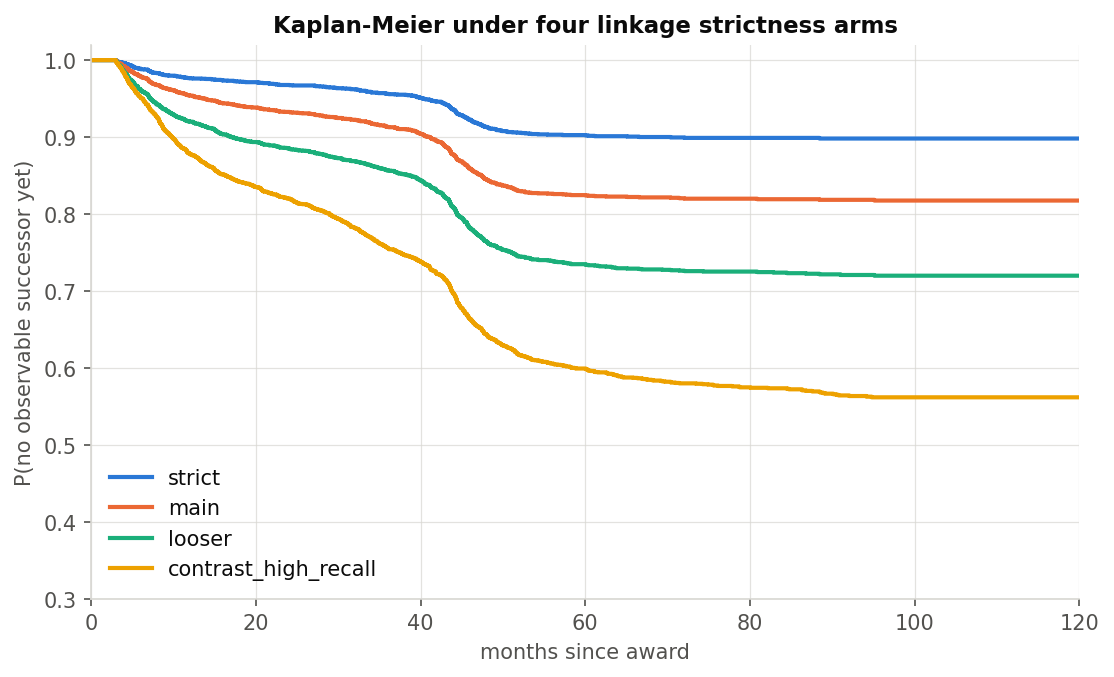
\includegraphics[width=0.85\linewidth]{figures/fig04_linkage_sensitivity.png}
\caption{Kaplan--Meier curves under the four retained linkage arms. The event count runs from 296 to 1,332 and the curves shift vertically, but they keep the same shape, including the 40--48 month shoulder. This is the report's central interpretive figure: absolute levels are conditional on the linkage rule, while the shape of the risk profile is not.}
\label{fig:sens}
\end{figure}


\textbf{(b) Borderline band.} The most fragile decisions are those whose best candidate sits near the bar. Removing the 280 episodes scoring in \([0.65; 0.75]\) --- a symmetric band fixed a priori and never searched over --- drops 133 events and gives: P($\le$ 12 m) 4.62 \% $\rightarrow$ 3.72 \%, CPV-35 HR 1.553 $\rightarrow$ \textbf{1.780}, framework HR 1.751 $\rightarrow$ 1.616. Both headline hazard ratios keep their direction.

\textbf{(c) Template-risk re-censoring.} The first two tests move the acceptance bar. But the false-positive mechanism the linkage audit identified produces links well \textbf{above} it: French award notices carry long standardised framework boilerplate on which character n-grams score highly between unrelated objects, and \texttt{M\_B} ranks candidates independently per anchor, so one episode can be accepted for several anchors. Two observable signatures define the at-risk group: word-level similarity below 0.50 (65 links), or a successor shared with another anchor (127 links) --- together \textbf{173 of the 544 links (31.8 \%)}. Those anchors are \textbf{re-censored at the cut-off} rather than deleted, because that is the counterfactual a spurious link implies: the anchor had no observed successor and should contribute its full follow-up as censored exposure. Result: P($\le$ 12 m) falls to 2.64 \%, but CPV-35 HR = \textbf{1.541} and framework HR = \textbf{1.692}. This is the test the framework finding most needed, since that boilerplate is the very text driving the mechanism.

\textbf{(d) Detectability.} The largest imbalance between linked and censored episodes is not a property of the contract at all:

\begingroup\footnotesize
\begin{longtable}[]{@{}lrrr@{}}
\toprule\noalign{}
Variable & Linked mean & Censored mean & SMD \\
\midrule\noalign{}
\endhead
\bottomrule\noalign{}
\endlastfoot
\textbf{log(candidate pool size)} & 4.787 & 3.972 & \textbf{+0.470} \\
candidate pool size & 274.3 & 188.6 & +0.285 \\
text length & 1,611 & 1,087 & +0.262 \\
framework flag & 0.265 & 0.187 & +0.187 \\
\end{longtable}
\endgroup

\texttt{M\_B} takes the maximum text score over the candidate block, and the maximum of more draws is larger: a buyer who publishes prolifically is mechanically more likely to yield an accepted link. This is an \textbf{observability} channel, not a cause of re-procurement. A sensitivity model adds \(\log(1 + \text{pool size})\):

\begingroup\footnotesize
\begin{longtable}[]{@{}lrrr@{}}
\toprule\noalign{}
Covariate & HR, main model & HR, + log(pool) & adjusted p \\
\midrule\noalign{}
\endhead
\bottomrule\noalign{}
\endlastfoot
Framework agreement & 1.751 & \textbf{1.617} & $2.6\times 10^{-6}$ \\
CPV-35 & 1.553 & \textbf{1.512} & $8.5\times 10^{-4}$ \\
log(pool size) & --- & 1.184 & $6.0\times 10^{-9}$ \\
\end{longtable}
\endgroup

Two readings follow, and they differ. \textbf{The population CPV-35 contrast is insensitive to direct pool-size adjustment}: the hazard ratio moves from 1.553 to 1.512 and remains directionally stable across event-definition checks. \textbf{The framework association is partly detectability}: roughly 14 \% of the log hazard ratio attenuates. Its direction remains positive across the main specifications, but its magnitude is smaller than the population model alone implies.

The main model is unchanged: this column is a sensitivity, not a new reference specification.

\textbf{(e) Buyer-stratified Cox.} Giving each buyer its own baseline hazard controls time-invariant buyer characteristics --- institutional procurement culture, region and persistent publication propensity among them. It does \emph{not} eliminate anchor-specific candidate-pool detectability: pool size varies within \textbf{473 of 514} buyers with multiple cohort episodes (92.0\,\%), because each anchor has a different award date and future follow-up. The pool-adjusted and buyer-stratified models therefore have distinct roles and neither replaces the other.

\begingroup\footnotesize
\begin{longtable}[]{@{}lrrr@{}}
\toprule\noalign{}
Within-buyer covariate & HR & 95\,\% CI & $p$ \\
\midrule\noalign{}
\endhead
Framework agreement & 1.497 & {[}1.150; 1.948{]} & 0.0027 \\
CPV-35 (ref. CPV-32) & 1.213 & {[}0.866; 1.699{]} & 0.262 \\
CPV-48 & 0.482 & {[}0.346; 0.672{]} & $1.7\times10^{-5}$ \\
CPV-72 & 0.831 & {[}0.627; 1.100{]} & 0.196 \\
Award year (centred) & 1.015 & {[}0.967; 1.065{]} & 0.547 \\
\bottomrule\noalign{}
\end{longtable}
\endgroup

The estimands now separate cleanly. At the Grand Ouest population level, CPV-35 episodes show earlier observable successors; within a buyer, the estimate attenuates toward 1 and is imprecise, suggesting that part of the population difference is compositional without proving confounding or refuting the population result. Framework status remains positive and statistically supported in the primary within-buyer analysis, although its magnitude attenuates; the strict event-definition arm is positive but imprecise. Buyer-stratified sensitivity also suggests slower observable-successor timing for CPV-48 within buyers. That direction is consistent across the four linkage arms, but it emerged from a sensitivity analysis and is treated as an \textbf{exploratory secondary result}, with no multiplicity-adjusted significance claim.

\subsection{What the survival analysis establishes}

Under the retained event definition, the probability that an awarded Grand Ouest digital procurement episode shows an observable successor is estimated at 4.6 \% by twelve months and 6.7 \% by twenty-four, with a marked re-procurement shoulder between 36 and 48 months. Absolute successor levels are strongly sensitive to the linkage definition, whereas several comparative patterns are more stable. At population level CPV-35 episodes show earlier successors, but the contrast attenuates within buyer; framework status remains positively associated after direct detectability and primary within-buyer controls; and the CPV-48 within-buyer slowdown is exploratory. The out-of-time point estimate is close to chance and does not establish useful individual ranking, so the Cox model is not used for that purpose.
